% vim: set tw=0:
\documentclass{beamer}
\usepackage{graphicx}
\usepackage{hyperref}
\hypersetup{pdfborder={0 0 0 0}}

% Reasonable themes:
% Antibes Bergen Berkeley Berlin Frankfurt Goettingen Ilmenau Luebeck Malmoe
% Montpellier PaloAlto Rochester Singapore Szeged Warsaw bars boxes
% compatibility default lined plain shadow sidebar split tree
% And these ones include the author's name on every slide:
% Berkeley

% Declare themes.
\mode<presentation>
\usetheme{UWHEP}

% Personal macros.
\newcommand{\email}[1]{{\texttt #1}}
\newcommand{\newframe}[1]{\section{#1}
    \frametitle{\sc{#1}}}
\newcommand{\subframe}[1]{\subsection{#1}
    \frametitle{\sc{#1}}}
\newcommand{\supers}[1]{\ensuremath{^\textrm{#1}}}
\newcommand{\subs}[1]{\ensuremath{_\textrm{#1}}}
\newcommand{\ca}{\ensuremath{\sim}}
\renewcommand{\email}[1]{\href{mailto:#1}{\nolinkurl{#1}}}

% Author information.
\title{T2 Status}
\author[Maier, Mohapatra]{
    Will Maier \and Ajit Mohapatra\\
    {\tt wcmaier@hep.wisc.edu}\\
    {\tt ajit@hep.wisc.edu}}
\institute[Wisconsin]{University of Wisconsin - High Energy Physics}
\date{2010.05.25}
\logo{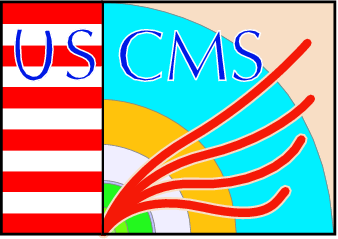
\includegraphics[height=0.6cm]{../../../Graphics/USCMS_logo.png}\hspace{.1cm}
\includegraphics[height=0.75cm]{../../../Graphics/UW_logo.png}}

\begin{document}

\begin{frame}
    \titlepage
\end{frame}

%\section{Overview}
%\begin{frame}
%    \tableofcontents
%\end{frame}

\section{Facilities}
\subsection{Software and Storage}
\begin{frame}
\frametitle{}

\begin{itemize}
	\item dCache: from the frying pan and into the fire
	\begin{itemize}
		\item One week of calm after resolving replication bug
		\item Then, PNFS server regularly overloaded
		\item Backed up queues, transfer timeouts
		\item Decreasing number of queues, tuning Postgres memory, tweaking dCache config, switching to fast PNFS didn't help
		\item Ultimately, traced problem to user workflow creating thousands of files in a few directories
		\item Modified local analysis scripts to limit number of outputs per directory, run smaller batches of jobs
		\item Chimera not affected? We plan to upgrade after ICHEP
	\end{itemize}
	\item Benchmarking CMSSW on new Opteron 6136 systems (2x8 2.40 GHz)
	\begin{itemize}
		\item Performance slightly slower than recent Xeons (with higher clockspeed)
		\item Not sure why runtimes spike at x=5, 9 and 12
		\item Scripts, data, plot available~\footnote{~\url{http://www.hep.wisc.edu/~wcmaier/performance/}}
	\end{itemize}
	\item Switched (finally) to GOC CA bundle
\end{itemize}
\end{frame}

\subsection{Production and Monitoring}
\begin{frame}
\frametitle{}

\begin{itemize}
	\item JobRobot: PNFS issues
	\item SAM: PNFS issues
	\item RSV: PNFS issues
	\item PhEDEx:
	\begin{itemize}
		\item Still holding on to 3\_3\_0 in Prod and Debug instances
		\item Disabled LT transfers from the problematic T2s in LCG
		\item Otherwise stable LT transfers, and usual MC/data transfers for local users
	\end{itemize}
	\item MC Production:
	\begin{itemize}
		\item Spring10 production (FullSim, FastSim and Data-like-MC) going on very well
		\item Preparing for some large scale Pile-up production at the T2s to see how the sites perform or if there are any issues
	\end{itemize}
\end{itemize}
\end{frame}
\end{document}
